\scanpage{313}
\uline{Séparation} de $\uline{\mathrm{Pic}}_{X/S}$

(i) Séparé sur $S$ si $X_s$ sont géom$^t$ loc. intègres ?

(ii) $\uline{\mathrm{Pic}}^\tau_{X/S}$ séparé sur $S$ si les $X_s$ séparables ?

${}_n\uline{\mathrm{Pic}}_{X/S}$ \qquad `` \qquad `` \qquad ?

\uline{N.B.} 1) Exemple de Mumford par des ``schémas en courbes elliptiques'', à fibre double, montre que $\uline{\mathrm{Pic}}^0_{X/S}$ peut ne pas être séparé sur $S$.
\margin{(mais alors il n'est pas représentable}

2) Exemple de
\figure{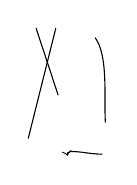
\begin{tikzpicture}[x=1cm,y=1cm]
\draw (0,0)--(.35,1.4);\draw (.1,1.4)--(.38,.55);
\draw (.85,1.28)..controls(1.02,1.05)and(.96,.5)..(.98,.2);
\draw[->](.94,-.2)..controls(.75,-.2)and(.48,-.12)..(.5,-.22);
\end{tikzpicture}}
montre que, $=$ si les fibres sont séparables, $\uline{\mathrm{Pic}}_{X/S}$ n'est pas tjrs \unsure{davantage} séparé sur \unsure{la|$S$}

\uline{Variation de} $\alpha,\lambda,\mu$.

(i) Constance de $\dim\uline{\mathrm{Pic}}_{X_s/k(s)}=\alpha_s+\mu_s+\lambda_s$ ?

(ii) $\alpha\leq\alpha'$, $\lambda\geq\lambda'$, \quad [$2\alpha+\mu\leq2\alpha'+\mu'$ connu]

\margin{du moins pour fibres séparables}

Soient $X,Y$ propres sur $S$, à fibres géom. intègres. Le préschéma. $\uline{\mathrm{Corr}}_S(X,Y)$ [classes de correspondances] existe-t-il ? \uuline{Oui}, par Raynaud ...
\mspage{312}
